\documentclass[a4paper,overfullrule=true]{scrartcl}

% Uncomment to optimize for double-sided printing.
% \KOMAoptions{twoside}

% Set binding correction manually, if known.
% \KOMAoptions{BCOR=2cm}

% Typographic niceties fixing a multitude of potential small issues
\usepackage{microtype}

% Localization options
\usepackage[english]{babel}
\usepackage[T1]{fontenc}
\usepackage[utf8]{inputenc}

% Quotations
\usepackage{dirtytalk}

% Enhanced verbatim sections. We're mainly interested in
% \verbatiminput though.
\usepackage{verbatim}

% PDF-compatible landscape mode.
% Makes PDF viewers show the page rotated by 90°.
\usepackage{pdflscape}

% Subfigures
\usepackage{subcaption}

% Figures at end (of chapter via \processdelayedfloats)
% \usepackage[figuresonly,nomarkers,nofiglist]{endfloat}

% Advanced tables
\usepackage{tabu}
\usepackage{longtable}

% Fancy tablerules
\usepackage{booktabs}

% Graphics
\usepackage{graphicx}

% Current time
\usepackage[useregional=numeric]{datetime2}

% Float barriers.
% Automatically add a FloatBarrier to each \section
\usepackage[section]{placeins}

% Importing CSV into tables
\usepackage{csvsimple}

\usepackage{geometry}
\usepackage{layout}

% Math tools
\usepackage{mathtools}
% Math symbols
\usepackage{amsmath,amsfonts,amssymb}
\usepackage{amsthm}

\DeclarePairedDelimiter\abs{\lvert}{\rvert}

\pagestyle{plain}
 
% Source code & highlighting
\usepackage{listings}

% SI units
\usepackage[binary-units=true]{siunitx}
\DeclareSIUnit\Molar{\textsc{m}}
\DeclareSIUnit\Da{\textsc{Da}}
\DeclareSIUnit\mole{mol}
\DeclareSIUnit\rpm{rpm}
\DeclareSIUnit\cfu{cfu}

\usepackage[version=4]{mhchem}

\newcommand{\odbact}{$\text{OD}_{600}$}

\newcommand{\mysubject}{2115 - Lab course biochemistry 2}
\newcommand{\mytitle}{Expression, purification and characterization of superoxide oxidase SOO}

% Convenience commands
\newcommand{\mailsubject}{\mysubject{} \mytitle{}}
\newcommand{\maillink}[2]{\href{mailto:#1?subject=\mailsubject}
                               {#2}}

% Should use this command wherever the print date is mentioned.
\newcommand{\printdate}{\today}

\subject{2115 - Lab course biochemistry 2}
\title{Expression, purification and characterization of superoxide oxidase `SOO'}
\subtitle{Final report}
\author{\maillink{michael.senn@students.unibe.ch}{Michael Senn} - 16-126-880}

\date{\printdate}

\publishers{von Ballmoos group, University of Bern\\Abbas Maxime Abou Hamdan \& Sabina Deutschmann}

% Needs to be the last command in the preamble, for one reason or
% another. 
\usepackage{hyperref}

\begin{document}
\maketitle

\begin{abstract}
	Three variants of superoxide oxidase were grown in bacterial BL21 cells
	and purified using size-exclusion and affinity chromatography.
	Purification efficiency was monitored using fluorescence of
	dsRed-tagged proteins.

	Purified enzymes were reconstituted into liposomes using freeze-thaw
	cycles. Reconstituted and solubilzed enzymes were then analyzed,
	measuring their reduction in presence of superoxide or quinone, as well
	as enzymatic activity using absorbance measurements.

	Using the collected data the enzymes were characterized, estimating
	their $K_m$ value as well as gaining insights into the orientation of
	enzymes in liposomes.
\end{abstract}

\newpage
\part*{Introduction}

Reactive oxygen species (`ROS') such as superoxide (\ce{O2-}) or hydrogen
peroxide (\ce{H2O2}) are toxic to the body, causing damage to proteins or DNA,
with links to various diseases including cancer. As such organisms under
aerobic conditions counteract ROS via eg Superoxide Dismutase (`SOD') which
catalyzes the partitioning of superoxide into molecular oxygen and hydrogen
peroxide.

One major source of superoxide is the oxidative phosphoryliation within the
mitochondrial matrix. \cite{Novo2008} To a lesser extent these superoxides
diffuse into the cytoplasm, where they are acted upon by SOD. A significant
portion of superoxides however is oxidised by superoxide oxidases - henceafter
referred to as `SOO' or `Halonsaft' due to its colour - a family of
membrane-bound proteins which oxidize superoxides.\cite{superoxide_salvaging}.

One protein of this family is CybB from E. Coli which was shown to function as
a superoxide:ubiquinone oxidoreductase. It oxidizes superoxide to oxygen while
simultaneously reducing quinone to quinol.\cite{superoxide_salvaging} This
enzymatic activity both serves to remove superoxides in close proximity to the
cell membrane, as well as restore the quinone pool, helping to save energy.

% TODO
% - Characterizing (eg activity) we did?
% - Transformation & expression basics

\newpage
\part*{Material \& methods}

\section{Transformation \& expression}

Transformation and expression were done as described.
\cite{superoxide_salvaging}. Summarily, \ce{CaCl2} treated cells were mixed
with pET28-cybB561 plasmids, and heat shock treated (\SI{30}{\min} on ice,
\SI{1}{\min} at \SI{42}{\celsius}, \SI{5}{\min} on ice, \SI{1}{\hour} at
\SI{37}{\celsius} shaking at \SI{900}{rpm}), then incubated overnight at
\SI{37}{\celsius} with \SI{30}{\ug\per\ml} Kanamycin. Transformed colonies were
picked and incoluated overnight at \SI{37}{\celsius} in LB medium with
\SI{30}{\ug\per\ml} Kanamycin and \SI{35}{\ug\per\ml} Chloramphenicol.

% TODO: Antibiotic amounts correct? Check lab journal

\section{Membrane isolation \& enzyme purification}

Purification of SOO was done as described. \cite{superoxide_salvaging}.

In summary, resuspended bacterial cells were broken open and DNASE-treated in a
maximator (3 passes at $>$\SI{1000}{\bar}). Pelleted membranes were resuspended
in \SI{50}{\milli\Molar} HEPES pH 7.5, \SI{200}{\milli\Molar} \ce{NaCl},
\SI{7.5}{\percent} glycerol buffer. Protein concentration was determined with a
BCA assay.

Membranes were solubilized in \SI{1}{\percent} OGNG \SI{1}{\milli\Molar} PMSF
and stirred at \SI{4}{\celsius} for \SI{1}{\hour}. Insolubilized membranes were
pelleted at \SI{150000}{g} for \SI{45}{\min}. The supernatant was loaded on a
\ce{Ni^{2+}} column and incubated for \SI{45}{\min} at \SI{4}{\celsius} on a
rotating wheel. The column was then washed and eluted with \SI{5}{\milli\Molar}
and \SI{100}{\milli\Molar} Histidine.

Parts of cybB561-dsRed were treated overnight with TEV-protease, and a reverse
\ce{Ni^{2+}} IMAC performed.

The eluate was concentrated to \SI{0.5}{\ml} with a \SI{10}{\kilo\Da}
concentrator, and loaded onto a S200 increase 10/300 column. Fractions
suspected to contain the protein were pooled. Protein concentration was
determined via absorbance mesurement of oxidized and reduced form (via addition
of DTT) between \SIrange{600}{400}{\nm}.

Aliquots of the purification steps were loaded onto a \SI{12}{\percent}
SDS-PAGE gel, ran at \SI{125}{\V} for \SI{20}{\min} and \SI{185}{\V} for
\SI{80}{\min}. The gel was stained with coomassie.

Efficiency of purification was measured via fluorescence measurement of
cyB561-dsred at an emission of \SI{586}{\nm} and extinction of \SI{555}{\nm}.

\section{Enzyme characterization}

Characterization was performed according to the same Nature
article\cite{superoxide_salvaging}.

Dried lipis were resuspended in \SI{20}{\milli\Molar} HEPES pH 7.4,
\SI{20}{\milli\Molar} \ce{KCl}, \SI{200}{\milli\Molar} \ce{NaCl}. Unliamellar
liposomes were formed by freeze-thaw cycles in nitrogen and \SI{29.4}{\celsius}
respectively, followed by sonication (\SI{2.5}{\min}, cycles of \SI{0.5}{\min}
on \SI{0.5}{\min} off).

CybB was reconstituted by adding enzymes to liposomes with \SI{0.6}{\percent}
sodium cholate. Detergent was removed by loading the sample on a P10 gel
filtration column and eluting it.

Reduction of CybB was measured via absorption measurement at \SI{428}{\nm}. In
a first set \SI{1}{\micro\Molar} of solubilized enzyme was mixed with
\SI{20}{\milli\Molar} HEPES ph 7.4, \SI{20}{\milli\Molar} \ce{KCl},
\SI{200}{\milli\Molar} \ce{NaCl}, \SI{0.05}{\percent} DDM for a final reaction
volume of \SI{750}{\ul}. At t=\SI{1}{\min} \SI{1}{\ul} substrate (quinol or
superoxide via Xanthyloxidase) was added, at t=\SI{3}{\min} the enzyme was
fully reduced via DTT. In a second set the same experiment was performed with
\SI{10}{\ul} reconstituted enzymes in equal fashion except a buffer without
detergent was used. The two sets were done for both the wildtype as well as the
mutant.

Fluorescence of reconstituted and solubilized, cleaved and uncleaved CybB-sred
was measured at excitation of \SI{555}{\nm} and emission of \SI{595}{\nm}.
Fluorescence was quenched with \ce{Cu2+} and restored with EDTA.

Activity of solubilized enzymes was determined by measuring reduction of WST-1
via absorption at \SI{455}{\nm}. In a first set \SI{100}{\micro\Molar} quinone,
\SI{60}{\nano\Molar} BO3 oxidase and buffer (\SI{100}{\milli\Molar} sodium
phosphate pH 8, \SI{0.1}{\milli\Molar} DTPA, \SI{0.1}{\milli\Molar}
Hypoxanthine, \SI{0.05}{\percent} DDM) for a final volume of \SI{750}{\ul} were
mixed. At t=\SI{0.5}{\min} \SI{0.03}{U} XO, at t=\SI{1.5}{\min} varying volumes
of enzyme were added. Enzyme concentration was increased until quenching of
superoxide production was level with a reference measurement done using
superoxide dismutase.

In a second set the determined concentration of enzyme was kept constant while
quinone concentration was varied.

\newpage
\part*{Results \& discussion}

\section{Transformation}

The goal of bacterial transformation was to get competent E. Coli cells of the
LEMO21 (DE3) strain to take up pET28a-cybB561 plasmids, allowing for the
selective overexpression of HS in presence of lactose or IPTG. Rhamnose allowed
to selectively inhibit the T7 polymerase translating the HS gene.
\cite{memstar} To permit selection the plasmid further encodes for a resistance
to kanamycin.

The overnight incubated plates containing kanamycin had multiple colonies
growing on them the next day. This showed that the heat shock treatment had
been successful,

\section{Expression}

\subsection{Expression monitoring}

During expression the efficiency of several media was to be established, both
in terms of speed of cell growth as well as yield of HS per cell. Three
different types of medium (LB, TB, ZYM-505) were prepared, with four samples
each.

Increasing the amount of produced proteins per cell was of interest as it
lowers the amount of detergent required to solublize the cell membranes.

Protein expression was monitored by measurement of \odbact of incubating
samples, visualized in figure \ref{fig:absorption_expression}. A mesurement at
\SI{90}{\min} was excluded as it had been done incorrectly. IPTG was added at
\SI{90}{\min}.

It was shown that cells grew faster in TB and ZYM-505 medium than in LB medium,
as seen by the slope of the curve as well as final \odbact reached.

It was further shown that samples not containing IPTG followed the normal
growth pattern of bacterial cells, starting in a lag phase of little cell
growth, a log phase of exponential cell growth - shown as a lineare incrase of
\odbact - and the beginnings of a stationary phase where cell growth cedes. The
absence of IPTG will have prevented overexpression of HS, allowing cells to
grow as normal.

Cells treated with IPTG at \SI{90}{\min} and not containing Rhamnose showed
stagnation of cell growth indicative of overexpression of HS. Cells treated
with IPTG and containing Rhamnose did not show any sign of overexpression of
HS.

\subsection{Expression efficiency}

After expression the amount of expressed HS-Dsred was measured via fluorescence
measurements. Results were normalized to cell density, giving an approximation
of protein concentration per cell. Such normalized results are are shown in
figure \ref{fig:fluorescence_expression}.

\subsubsection{Base protein expression}

Overall protein expression per cell can be estimated using IPTG-negative
samples. It was shown that LB and ZYM-505 media produce comparable amounts of
proteins per cell, while the amount of proteins per cell in the TB medium was
significantly higher. This conflicts with the memstar paper which found that
protein production normalized to cell density was only slightly higher in TB
compared to the other two media. \cite{memstar}

It is possible that the cell density of the TB samples was underestimated, as
the linear relation between \odbact and cell density only holds for low values
of \odbact, as well as the spectrophotometer being less accurate for values
exceeding $1$.

\subsubsection{HS-Dsred expression}

Comparing the normalized fluorescence of IPTG-positive, Rhamnose-negative
samples with other samples in the same media showed that addition of IPTG
increased the amount of proteins - specifically HS-Dsred - which was expressed
per cell.

\subsubsection{Limiting HS-Dsred expression with Rhamnose}

Addition of Rhamnose to samples was supposed to limit the overexpression of
HS-Dsred, preventing a coplete stagnation of cell growth as well as the
potential buildup of inclusion bodies. \cite{memstar}.

As Rhamnose-positive samples did not show any sign of HS-Dsred expression, with
fluorescence levels comparable to IPTG-negative samples, we conclude that
either too much Rhamnose was added such that the T7 polymerase was inhibited
fully, or that no IPTG had been added to those samples.


\begin{figure}
	\centering
	\begin{subfigure}{\textwidth}
		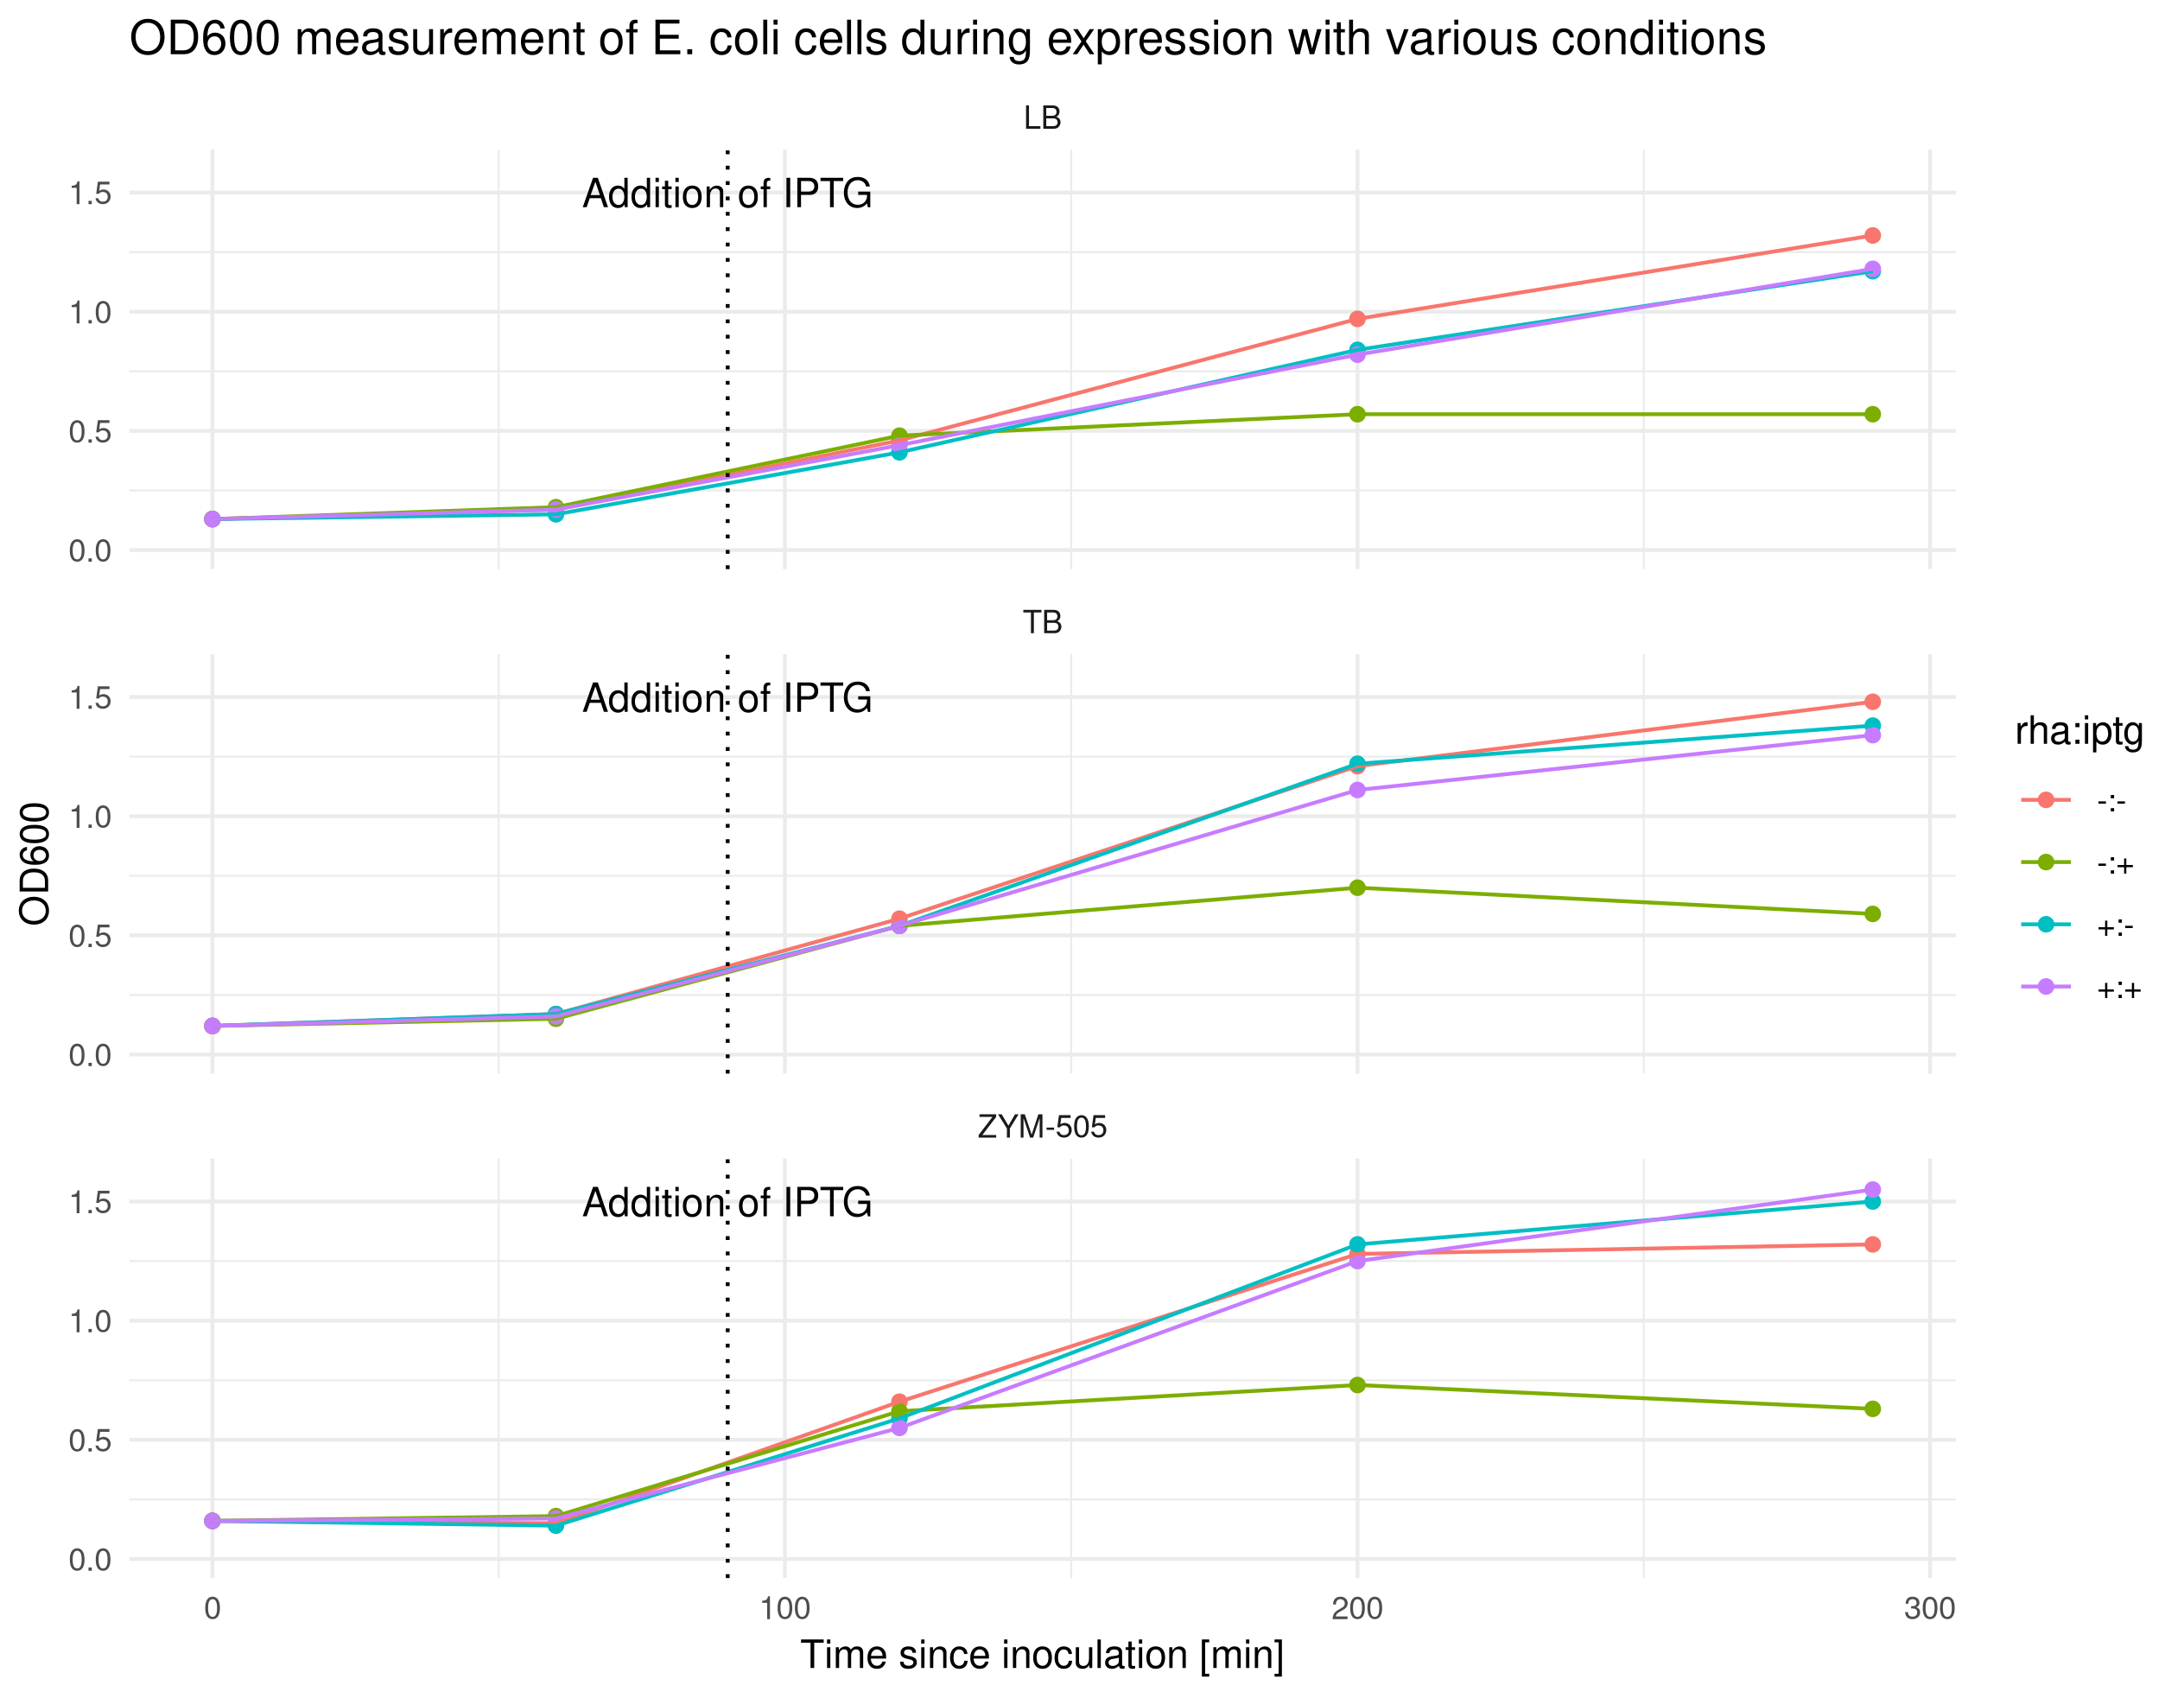
\includegraphics[width=0.8\linewidth]{../img/absorption_expression.png}
		\caption{\odbact values over time during protein expression}
		\label{fig:absorption_expression}
	\end{subfigure}

	\begin{subfigure}{\textwidth}
		\centering
		\includegraphics[width=0.8\linewidth]{../img/expression_fluorescence.png}
		\caption{Fluorescence of samples after protein expression}
		\label{fig:fluorescence_expression}
	\end{subfigure}

	\caption{Monitoring speed and efficiency of expression}
	\label{fig:expression}
\end{figure}


\section{Purification}

% Protein concentration


\section{Characterization}


\newpage
\part*{Conclusion}

% Issues with:
% - Expression: TB expression amount, IPTG+/Rha+,


\newpage
\bibliographystyle{plain}
\bibliography{references}

\end{document}
